% ===========================================
% Template for ICMC 2016 (version2)
% adapted from earlier LaTeX paper templates for the ICMC, SMC, etc...
% ===========================================

\documentclass{article}
\usepackage{icmc2016template}
\usepackage{times}
\usepackage{ifpdf}
\usepackage{soul}
\usepackage[english]{babel}
%\usepackage{cite}
\usepackage{amsfonts}
%\usepackage{todonotes}

\newcommand{\hilite}[1]{\colorbox{yellow}{#1}}
\long\def\todo#1{\hilite{{\bf TODO:} {\em #1}}}


%%%%%%%%%%%%%%%%%%%%%%%% Some useful packages %%%%%%%%%%%%%%%%%%%%%%%%%%%%%%%
%%%%%%%%%%%%%%%%%%%%%%%% See related documentation %%%%%%%%%%%%%%%%%%%%%%%%%%
%\usepackage{amsmath} % popular packages from Am. Math. Soc. Please use the 
%\usepackage{amssymb} % related math environments (split, subequation, cases,
%\usepackage{amsfonts}% multline, etc.)
%\usepackage{bm}      % Bold Math package, defines the command \bf{}
%\usepackage{paralist}% extended list environments
%%subfig.sty is the modern replacement for subfigure.sty. However, subfig.sty 
%%requires and automatically loads caption.sty which overrides class handling 
%%of captions. To prevent this problem, preload caption.sty with caption=false 
%\usepackage[caption=false]{caption}
%\usepackage[font=footnotesize]{subfig}

% ====================================================
% ================ Define title and author names here ===============
% ====================================================
%user defined variables
\def\papertitle{Recursive Generation of Rhythmic Structures with PTGGs}
\def\firstauthor{Brian Heim}
\def\secondauthor{Donya Quick}

% adds the automatic
% Saves a lot of output space in PDF... after conversion with the distiller
% Delete if you cannot get PS fonts working on your system.

% pdf-tex settings: detect automatically if run by latex or pdflatex
\newif\ifpdf
\ifx\pdfoutput\relax
\else
   \ifcase\pdfoutput
      \pdffalse
   \else
      \pdftrue
  \fi
\fi

\ifpdf % compiling with pdflatex
  \usepackage[pdftex,
    pdftitle={\papertitle},
    pdfauthor={\firstauthor, \secondauthor},
    bookmarksnumbered, % use section numbers with bookmarks
    pdfstartview=XYZ % start with zoom=100% instead of full screen; 
                     % especially useful if working with a big screen :-)
   ]{hyperref}
  %\pdfcompresslevel=9

  \usepackage[pdftex]{graphicx}
  % declare the path(s) where your graphic files are and their extensions so 
  %you won't have to specify these with every instance of \includegraphics
  \graphicspath{{./figures/}}
  \DeclareGraphicsExtensions{.pdf,.jpeg,.png}

  \usepackage[figure,table]{hypcap}

\else % compiling with latex
  \usepackage[dvips,
    bookmarksnumbered, % use section numbers with bookmarks
    pdfstartview=XYZ % start with zoom=100% instead of full screen
  ]{hyperref}  % hyperrefs are active in the pdf file after conversion
  \usepackage[dvips]{epsfig,graphicx}
  % declare the path(s) where your graphic files are and their extensions so 
  %you won't have to specify these with every instance of \includegraphics
  \graphicspath{{./figures/}}
  \DeclareGraphicsExtensions{.eps}

  \usepackage[figure,table]{hypcap}
\fi

%setup the hyperref package - make the links black without a surrounding frame
\hypersetup{
    colorlinks,%
    citecolor=black,%
    filecolor=black,%
    linkcolor=black,%
    urlcolor=black
}


% ====================================================
% ================ Title and author info starts here ===============
% ====================================================
% Title.
% ------
\title{\papertitle}

% Authors
% Please note that submissions are anonymous, therefore 
% authors' names should not be VISIBLE in your paper submission.
% They should only be included in the camera-ready version of accepted papers.
% uncomment and use the appropriate section (1, 2 or 3 authors)
%
% Single address
% To use with only one author or several with the same address
% ---------------
%-------------
\twoauthors
 {1.5in}
 {\firstauthor} {Yale University \\  %
   {\tt \href{mailto:brian.heim@yale.edu}{brian.heim@yale.edu}}}
 {\secondauthor} {Southern Methodist University \\  %
   {\tt \href{mailto:dquick@mail.smu.edu}{dquick@mail.smu.edu}}}


% ====================================================
% =============== The document content starts here ===============
% ====================================================
\begin{document}
%
\capstartfalse
\maketitle
\capstarttrue
%
\begin{abstract}
We present an approach for generating passages of rhythm via the use of a probabilistic temporal graph grammar with rule sets that operate via recursive subdivision. This project is motivated by three factors: (1) the recognition that the literature on computer-generated rhythm is generally not as robust as those for melody and harmony; (2) the creation of more tools for computer-assisted composition; and (3) the hope that such an approach, having already produced compelling results for some styles of music, may provide insight into the structure of rhythms found in existing repertoires.
\end{abstract}

%%%%%%%%%%%%%%%%%%%%%%%%% Introduction %%%%%%%%%%%%%%%%%%%%%%%%%%%%%%%

\section{Introduction}\label{sec:introduction}

There has been extensive work in the areas of analyzing and generating pitch-related features in music such as \linebreak melody and harmony. However, rhythmic structure has received substantially less attention, particularly in the area of automated composition. Typically, generated rhythms are either very simple, such as those found in Bach chorales, or they struggle to retain a sense of meter. 

We present a grammatical approach to generating diverse rhythmic patterns in multiple time signatures while preserving hypermetrical structures. Our approach also allows the generation of repeated patterns at multiple levels of granularity, an extremely important feature of rhythm in music. Finally, the probabilistic grammars described here also have the potential for rule probabilities to be derived from a corpus of real musical examples.

As both authors are familiar with the Common Practice era of Western classical music, the model and examples presented here derive significantly from that corpus. A partial goal of the initial implementation of this approach was to aid in computer-assisted composition. Particular design choices were made in order to make idioms common in contemporary Western classical music easily accessible; the result of this may be seen in the ``complex'' example below (Figure \ref{example_complex}). In Future Work, we also discuss the possibility of adapting the implementation for features common to other genres of music.

\subsection{Related Work}

One of the most commonly applied algorithms in computer music analysis and generation is the Markov chain \cite{chordia2011, gillick2009, yi, pachet}. However, Markov chains are fundamentally limited in the temporal scope of features that they can capture, which is problematic for modeling metrical structure and rhythmic patterns---for which temporal context and repetition are extremely important. As the order of the chain increases, more complex features can be modeled, but observations of states become sparse and the number of states increases exponentially. Even approaches such as variable-length Markov chains \cite{ron, buhlmann} and the extensions noted above do not entirely overcome these problems.

Some extensions to Markov chains exist that can overcome some of the problems of preserving metrical structure observed with more traditional approaches. Roy and Pachet model meter in melodic generation \cite{roy2013} using an extension known as Markov constraints \cite{pachet2011} to achieve properties such as properly filled measures. This method involves enumeration of possible outcomes for metrical constraints, although the complexity is mitigated to some extent by a filtering step to avoid a truly brute force search.

Work such as that of Lerdahl and Jackendoff \cite{gttm}, as well as the work of Temperley \cite{temperley2010}, presents a statistical view of metrical structure, where metrical positions are assigned a probability distribution and downbeats are weighted more heavily. While these models are useful analytically and can be used to generate new rhythmic patterns, as with Markov chains, there is no support for modeling repetition, and relatively common, syncopated rhythmic patterns are unlikely due to having little downbeat content. 

Grammars fundamentally have more expressive power \linebreak than Markov chains, with some categories of grammar supporting long-term constraints and even repetition. Because of this, we feel that grammatical approaches are better \linebreak suited to modeling rhythm and metrical structure than \linebreak purely Markovian methods.

Keller and Morrison present a grammatical model for jazz solos that includes a rhythmic component\cite{keller}. This grammar is context-free and generates rhythmic structure independently of melodic structure. The rhythmic portion of the grammar is fundamentally based on dividing times in half. Although some degree of syncopation is supported, the strategy of halving durations through much of the generation fundamentally limits it to duple meters. The grammars we introduce in later sections of this paper use a tiered, multi-rule-set approach that supports many other time signatures. 

\subsection{Probabilistic Temporal Graph Grammars}

A grammar is defined as a 4-tuple: $G = (N,T,R,S)$ where the alphabet $N \cup T$ comprises nonterminals, $N$, and terminals, $T$. $R$ is a set of rules of the form $x \in N \rightarrow (N \cup T)^{*}$ and $S \in N$ is the starting symbol. Terminals are symbols that only produce themselves, i.e. cannot be further altered, while nonterminals may produce any combination of terminals and nonterminals. The condition that production rules operate on individual symbols without knowledge of the surrounding symbols means that this definition also describes a Context-Free Grammar (CFG). Probabilistic context-free grammars (PCFGs) have more than one rule with the same left-hand side. Rules sharing the same left-hand side in a PCFG must have associated probabilities that sum to 1.0.

Kulitta features a category of grammars called Probabilistic Temporal Graph Grammars\cite{quick2013farm, quick_thesis}, or PTGGs. PTGGs are essentially parameterized PCFG, where production \linebreak rules are functions on parameters. Allowable functions on symbol parameters include simple conditional logic and let-in statements for variable creation and instantiation. \linebreak These let-in statements allow the generation of repetitions, which are an important feature of rhythm in music.

The generative algorithm used with PTGGs is similar to that of L-Systems: at each generative iteration of the grammar, starting with the single-symbol sequence of $X = S$, the appropriate rule $(x \rightarrow y) \in R$ is applied to each nonterminal symbol from left to right to produce a new sequence $X'$, which may contain more symbols than $X$. The sequence length is a nondecreasing function of the number of iterations. 


Rules in PTGGs have the following format:

$\;$ \\
\begin{tabular}{ll}
$x^p \rightarrow$ & $f_{1}(p)$ \\
$\;$ & $ \vert \;  \textbf{if} \; cond(p) \; \textbf{then} \; f_{1}(p) \; \textbf{else} \; f_{2}(p)$ \\
$\;$ & $\vert \; \textbf{let} \; x = f_{1}(p) \; \textbf{in} \; \{x \; | \; f_{i}(p)\}^{+}$ \\
\end{tabular} $\;$ \\

\noindent where each $f_{i}(p)$ indicates some function from parameter values to sequences of terminals and nonterminals and $cond(p)$ is a conditional test on the left-hand-side symbol's parameter (such as $p<2$).

%%%%%%%%%%%%%%%%%%%%%%%%% Grammar %%%%%%%%%%%%%%%%%%%%%%%%%%%%%%%

\section{A PTGG for Rhythm}

% substituted Roman numerals for ABCD - unfortunately people will complain that it looks like pitch classes.

In most PTGGs used by Kulitta, the alphabet consists of Roman numeral chord symbols parameterized by duration, and rules are \emph{duration preserving}, meaning that the right-hand side symbols divide up the duration of the left-hand symbol, typically by a power of two. This division always results in a string that has equal duration to the original symbol. A rule such as $I^{t} \rightarrow I^{t/2} V^{t/4} I^{t/4}$ indicates that a I-chord may be replaced by a I-V-I progression where the chord durations are $\frac{1}{2}$, $\frac{1}{4}$, and $\frac{1}{4}$ the durations of the original chord. This implies a general approach of beginning with a long duration and iteratively dividing it into progressively smaller durations; since one would typically like to have control over the exact duration of a generated composition, this is a reasonable approach.

The grammar proposed here is based on the observation that many theories of Western counterpoint, including those of Fux, Schoenberg, and Schenker \cite{fux_et_al, schoenberg}, treat rhythm as a hierarchy of nested structures, discuss metrical patterns such as anapest (short-short-long) in the same light regardless of the hierarchical level on which they occur, and regard small note values as elaborations or ornamentations of a less complex metrical pattern.

We also introduce the notion of \emph{production phases} into the PTGG framework to account for the need for different rules to take place at different granularities in the generative process.

Durations are treated as both terminals and nonterminals of an infinite parametrized alphabet of duration types in a four-phase generation algorithm process, each step of which subdivides an initial duration into smaller and \linebreak smaller units.

Throughout the following sections, we use $1.0$ to represent the duration of a whole note in 4/4.

\subsection{Nonterminals}

The nonterminals of the grammar are $N=\{Beat,\allowbreak Dotted,\allowbreak QuarterDotted,\allowbreak Measures \} \cup TS$ where $TS$ is a set of \emph{time signature symbols}. 


The \emph{Beat} symbol represents a note with duration $2^n/m$ where $n$ and $m$ are integers with $n \geq 0$, $m > 0$. The \emph{Dotted} symbol represents a duration analogous to a dotted note; it lasts $1.5$ times its undotted value. Similarly, a \emph{QuarterDotted} lasts for $1.25$ times its undotted value. Although the notion of a ``quarter dotted'' note has no counterpart in common practice notation (although some composers such as George Crumb have invented their own symbols for it), a duration of $\frac{5}{8}$ is found frequently in situations where, for example, a quarter note is tied to the first of a series of sixteenth notes. Because the grammar has no way to represent ties, this symbol is included for robustness.

One could argue that, for the sake of completion, symbols for $\frac{7}{8}$, $\frac{9}{8}$, and so on ought also to be defined. We have chosen to forego defining these symbols because (1) their durations occur less frequently than $\frac{3}{8}$ and $\frac{5}{8}$, (2) we are still able to express a wide variety of rhythms without them, (3) there are other, more elegant routes to the same solution (see Future Work).

% It was chosen to be a terminal for convenience, since any subdivision of a dotted value can also be articulated as a more complex subdivision of a longer duration.

\emph{Measures} represents a nonzero length of consecutive measures; each measure has nonzero duration but has not yet been assigned a time signature. Finally, $TS$ is the set of time signatures that may appear in the final output; symbols in $TS$ are named for the meters they represent: \emph{FourFour}, \emph{ThreeFour}, \emph{SixEight}, and so on. 
 
\subsection{Terminals}

% Note from Donya: this section had trouble displaying properly. Rewording eventually fixed it??? I have no idea why.
The set of terminals consists of one element: $T=\{Short\}$. \emph{Short} stands for a \emph{Beat} which has been subdivided to the point where its duration is less than or equal to $\frac{1}{2^n}$, where $n$ is an arbitrary integer constant. Intuitively, a very short note is prevented from being further subdivided. This behavior is designed to mimic the limits of human performers? rhythmic articulation.

The notations $B^d$, $S^d$, $D^d$, $Q^d$ will be used hereafter for $Beat$, $Short$, $Dotted$, and $QuarterDotted$ symbols of duration $d$ respectively. We also use the notation $M^l$ for a $Measures$ symbol with length $l$.

\subsection{Production Phases}

Production occurs in four phases of rule sets. A sentence is considered well-formed if and only if it passes through all four phases. These phases correspond to the generation of (1) phrase structure, (2) time signatures, (3) intra-measure beat patterns, and (4) recursive rhythmic subdivision. Having four separate rule sets, each with a well-defined purpose, allows us a great deal of flexibility without forcing us to over-specify.

Phase 1 begins with the string $\alpha = M^l$ where $l=2^a$, $a \geq 0$, and halts with the string $\beta = \{ M^1 \}^*, |\beta| = l$.

Phase 2 generates $\gamma$ from $\beta$ by replacing each $M^1$ in $\beta$ with a symbol $ts \in TS$, where $TS$ is a nonempty set of time signature symbols.

Phase 3 generates $\delta$ from $\gamma$ by replacing each $ts$ in $\gamma$ with a sequence of symbols from $\{Beat,\allowbreak Short,\allowbreak Dotted,\allowbreak QuarterDotted \}$ such that each sequence's duration sums to the duration of the time signature it replaces. For instance, the sequence
$[B^\frac{1}{2} D^\frac{3}{8} B^\frac{1}{8}]$ may be validly generated from \emph{FourFour} through the application of the third and then second rules in Table \ref{4_4rules}, 
%, because $\frac{1}{2} + \frac{3}{8} + \frac{1}{8} = 1$; % % removed - wasn't entirely correct for updated rule sets.
while the sequence $[B^\frac{1}{2} D^\frac{3}{4}]$, however, may not be generated from \emph{FourFour}.

Phase 4 generates the output string by repeatedly subdividing $\delta$. Rules in this phase operate within the duration-parametrized set $\{Beat,\allowbreak Short,\allowbreak Dotted,\allowbreak QuarterDotted \}$. In order to preserve the duration of $\delta$, the durations of the right-hand side of a rule must sum to the duration of the left-hand side.

% TODO: decide whether or not to keep this section

% \subsection{Sentential Forms}

% [Needs work - may be worth cutting]

% The set K of sentential forms of this PTGG is %, without considering parameter values, is

% $k \in K ::= M \; | k?k \; | \;  let \; x=k \; in \; k$

% \noindent for the first phase and 

% $l \in L ::= B \; | \; ( S \; | \; Dl \; | \;  lD \; | \; l?l ) \; | \;  let \; y=l \; in\;  l$

% %\noindent for the second, where $x \in V$, $y \in W$, and $V,W$ are predefined sets of variables.
% \noindent for the second, where $x$ and $y$ are variable names.

\subsection{Production Rules}

Production rules in Phase 1 are functions from measures to measure groups, $M \rightarrow K$, and in Phase 2 from beats to beat groups, $B \rightarrow L$. The strict definition of PFCG says that a single rule must produce a single string of symbols, as in the case of $B \rightarrow BB$ and $B \rightarrow SS$.  Yet \emph{Short}, as noted above, is only produced when its parameter meets certain conditions. Since the decision to output B, D or S can be made solely on the basis of the parameter value, we define rules as functions:

$B^a \rightarrow \mathbb{X} \in \mathbb{Q}^{p}$ where 

$p > 0 , \forall x \in X: 0 < x \leq 1, \sum_{x \in X} x = 1$

and then use the resulting parameters $[d_1,d_2,\ldots,d_p]=aX$ to label the produced symbols. In words, this means that the right-hand side is a list of fractions, summing to 1, that describe how the left-hand side is to be subdivided. This allows us to define patterns of subdivision clearly and succinctly. For example, let two Phase 4 rules be $B \rightarrow [\frac{3}{4}, \frac{1}{4}]$ and $B \rightarrow [\frac{1}{2}, \frac{1}{4}, \frac{1}{4}]$. Here are two iterations of production using these rules and a \emph{Short} threshold of $\frac{1}{16}$:

\bgroup
\def\arraystretch{1.5}
\begin{center}
\begin{tabular}{ l l }
 Rule & String \\
 \hline
 (start)                                                  & $B^{1}$ \\
 $B \rightarrow [\frac{3}{4}, \frac{1}{4}]$               & $D^{\frac{3}{4}} B^{\frac{1}{4}}$ \\
 $B \rightarrow [\frac{1}{2}, \frac{1}{4}, \frac{1}{4}]$  & $D^{\frac{3}{4}} B^{\frac{1}{8}} S^{\frac{1}{16}} S^{\frac{1}{16}}$ \\
\end{tabular}
\end{center}
\egroup

%%%%%%%%%%%%%%%%%%%%%%%%% Implementation %%%%%%%%%%%%%%%%%%%%%%%%%%%%%%%

\section{Implementation}

We use Haskell-based PTGG generation framework from Kulitta and the MIDI export capabilities offered by the Euterpea library \cite{euterpea} to allow for elegant rule definition and parsing. Below are some of the key features of this implementation.

\subsection{Four-Phase Generation Algorithm}

Assuming the rule sets have already been defined, the complete generation algorithm requires four parameters: (1) the total length $l = 2^n$, $n > 0$, of the passage in measures; (2) the shortest allowable duration $1/{2^s}$ expressed as $s$; (3) the number of Phase 4 iterations to perform; and (4) a random seed.

As stated above, generation begins with the string $\alpha = M^l$. Phase 1, phrase structure generation, uses only two rules: $M^l \rightarrow M^\frac{l}{2} M^\frac{l}{2}$ and $\textbf{let} x = M^\frac{d}{2} \textbf{in} x x$. Both rules subdivide the group of measures into two equal halves, but one does so through variable instantiation. Since $l$ is a power of two, Phase 1 halts in $log_2 l$ iterations.

In Phase 2, time signature assignment, each measure is assigned a time signature from the set $TS$. Since most pieces of common practice music are in a single time signature, this step will typically only consist of one rule $M \rightarrow ts$, $\{ ts \} = TS$.

In Phase 3, beat pattern assignment, each time signature symbol is replaced with a sequence of duration symbols that sum to the duration of that meter. An example Phase 3 rule might be $FourFour \rightarrow B^\frac{1}{2} B^\frac{1}{2}$, which divides a 4/4 measure into two independent halves. This Phase may also be trivial for generating common practice passages, but for complex or irregular time signatures such as 7/8, it is helpful to explicitly define the abstract beat pattern as $2 + 2 + 3$, or $3 + 2 + 2$, or even a mix of both.

Finally, Phase 4 replaces each duration symbol with a sequence of durations that sum to the original symbol's duration. The rules in Phase 4 are applied for a predetermined number of iterations. Each Phase 4 rule is actually a conditional predicated on the parameter of the left-hand side: the algorithm first determines if applying the subdivision would produce a duration shorter than the shortest allowed duration. If so, the symbol is left unchanged; otherwise, subdivision occurs, replacing symbols with $B$, $D$, or $S$ as described in Production Rules.

As a last step, a single measure consisting of a whole note or its equivalent in the relevant time signature is appended to the resulting string, in order to give a sense of finality.

%%%%%%%%%%%%%%%%%%%%%%%%% Examples %%%%%%%%%%%%%%%%%%%%%%%%%%%%%%%

\section{Examples}

We now present three example passages generated from this grammar. The first two are in 4/4 and 3/4 time respectively, with rule sets chosen freely in a rough attempt to imitate the repertoire of the Classical period of Western classical music. The third example is in a mix of irregular meters and demonstrates the ease of extending the grammar to a more contemporary style of rhythm, somewhere between the tuplets of Elliott Carter and Karlheinz Stockhausen and the dense rhythmic variety of Brian Ferneyhough. The purpose of these examples is primarily to give a sense of the variety and complexity possible under this approach, rather than to directly imitate any particular composer, school, or period. % In all probability tables shown here, it is implied that the parameter superscripts of the right-hand side subdivide the duration parameter of the left-hand side. % The exception to this rule is that when transforming a time signature symbol to a sequence of duration symbols, as in the rule $FourFour \rightarrow B^\frac{1}{2} B^\frac{1}{2}$, the right-hand side gives absolute parameter values, since there is in fact nothing to subdivide yet.

% The probability distribution between the two rules of Phase 1--whether to split using variable instantiation or not--can have significant consequences for the generated passage. If the probability of variable instantiation is $1$, every measure will look exactly the same; if it is $0$, every measure can develop independently. For all three examples we have used the distribution shown in Table \ref{4_4rules_phases123}: $0.33$ for variable instantiation, and $0.67$ otherwise. We can see the effect of this phase clearly in Figure \ref{example_3_4}. It is unlikely that that the first two measures would be subdivided in exactly the same way in later phases of generation, but with the variable instantiation introduced early on during Phase 1, they are guaranteed to be the same. With the same probability, the third and fourth measures could have matched, or the first two measures could have matched the last two. In this way, the purpose of Phase 1 is to introduce symmetry and structure probabilistically, in a way that feels similar to the structure of phrases in common practice music.

%%%%%%%%%%%%%%%%% 4/4 Example %%%%%%%%%%%%%%%%%%

\begin{figure*}[t] % NEEDS REPLACING BUT DEMOS MULTI-COLUMN SPAN
\centering
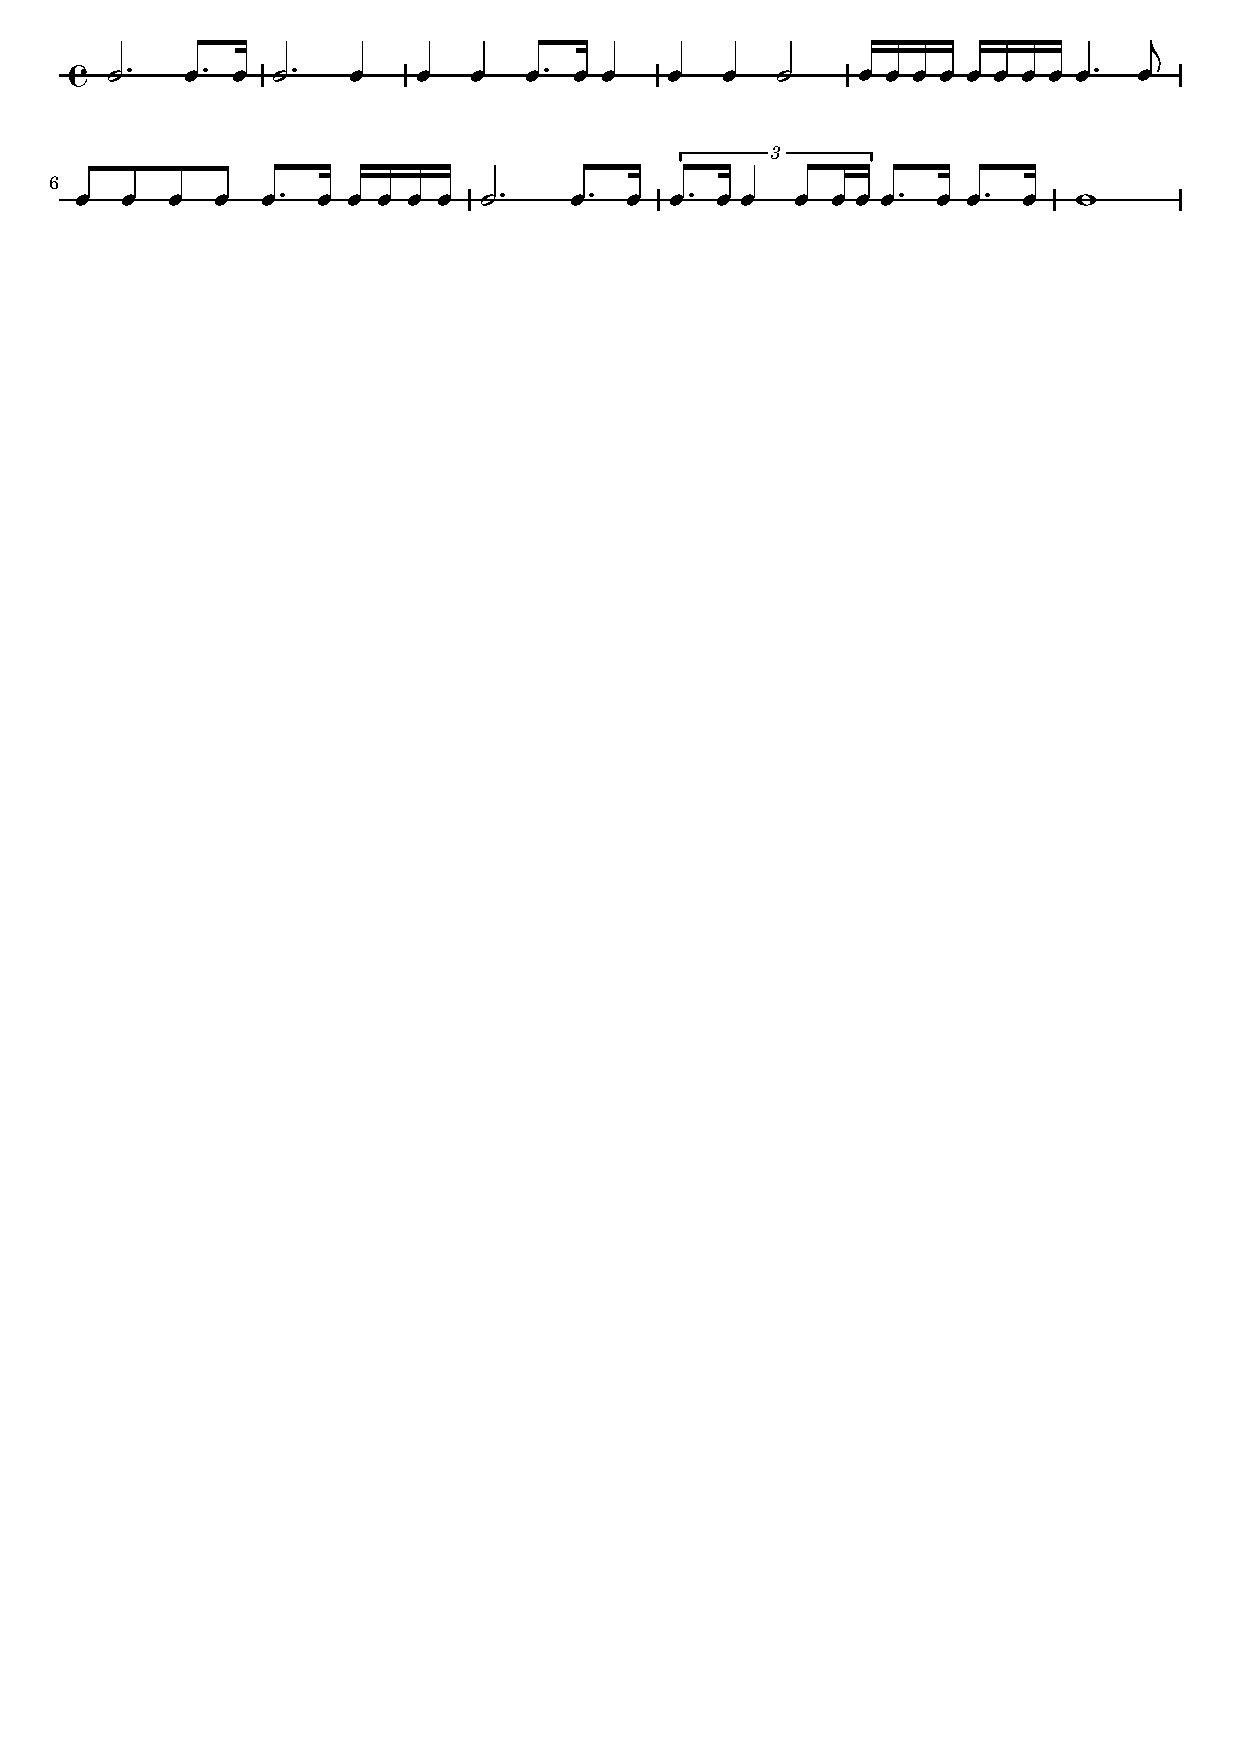
\includegraphics[width=16cm]{4_4_new.pdf}
\caption{A generated passage of eight measures of 4/4, with an extra whole note measure added for finality.}\label{example_4_4}
\end{figure*}

\begin{table}
\centering
\begin{tabular}{ll}
0.33 & $M \rightarrow \textbf{let} \; x = M^\frac{l}{2} \; \textbf{in} \; x \; x$\\
0.67 & $M \rightarrow M^\frac{l}{2} M^\frac{l}{2}$\\
1.00 & $M \rightarrow FourFour$\\
1.00 & $FourFour \rightarrow B^1$\\
\end{tabular}
\caption{Rules, along with their corresponding probabilities, used in Phases 1, 2 \& 3 to generate Figure \ref{example_4_4}}\label{4_4rules_phases123}
\end{table}

\begin{table}
\centering
\begin{tabular}{ll}
0.30 & $B \rightarrow B^1$\\
0.20 & $B \rightarrow D^\frac{3}{4} B^\frac{1}{4}$\\
0.15 & $B \rightarrow B^\frac{1}{2} B^\frac{1}{2}$\\
0.10 & $B \rightarrow B^\frac{1}{2} B^\frac{1}{4} B^\frac{1}{4}$\\
0.05 & $B \rightarrow B^\frac{1}{4} B^\frac{1}{2} B^\frac{1}{4}$\\
0.05 & $B \rightarrow B^\frac{1}{3} B^\frac{1}{3} B^\frac{1}{3}$\\
0.15 & $B \rightarrow \textbf{let} \; x = B^\frac{1}{2} \; \textbf{in} \; x \; x$\\ 
0.15 & $B \rightarrow \textbf{let} \; x = B^\frac{1}{4} \; \textbf{in} \; B^\frac{1}{2} \; x \; x$\\ 
1.00 & $D \rightarrow D^1$\\
\end{tabular}
\caption{Phase 4 rule set used to generate Figure \ref{example_4_4}.}\label{4_4rules}
\end{table}

%%%%%%%%%%%%%%%% 3/4 Example %%%%%%%%%%%%%%%%%%

\begin{figure*}[t] % NEEDS REPLACING BUT DEMOS MULTI-COLUMN SPAN
\centering
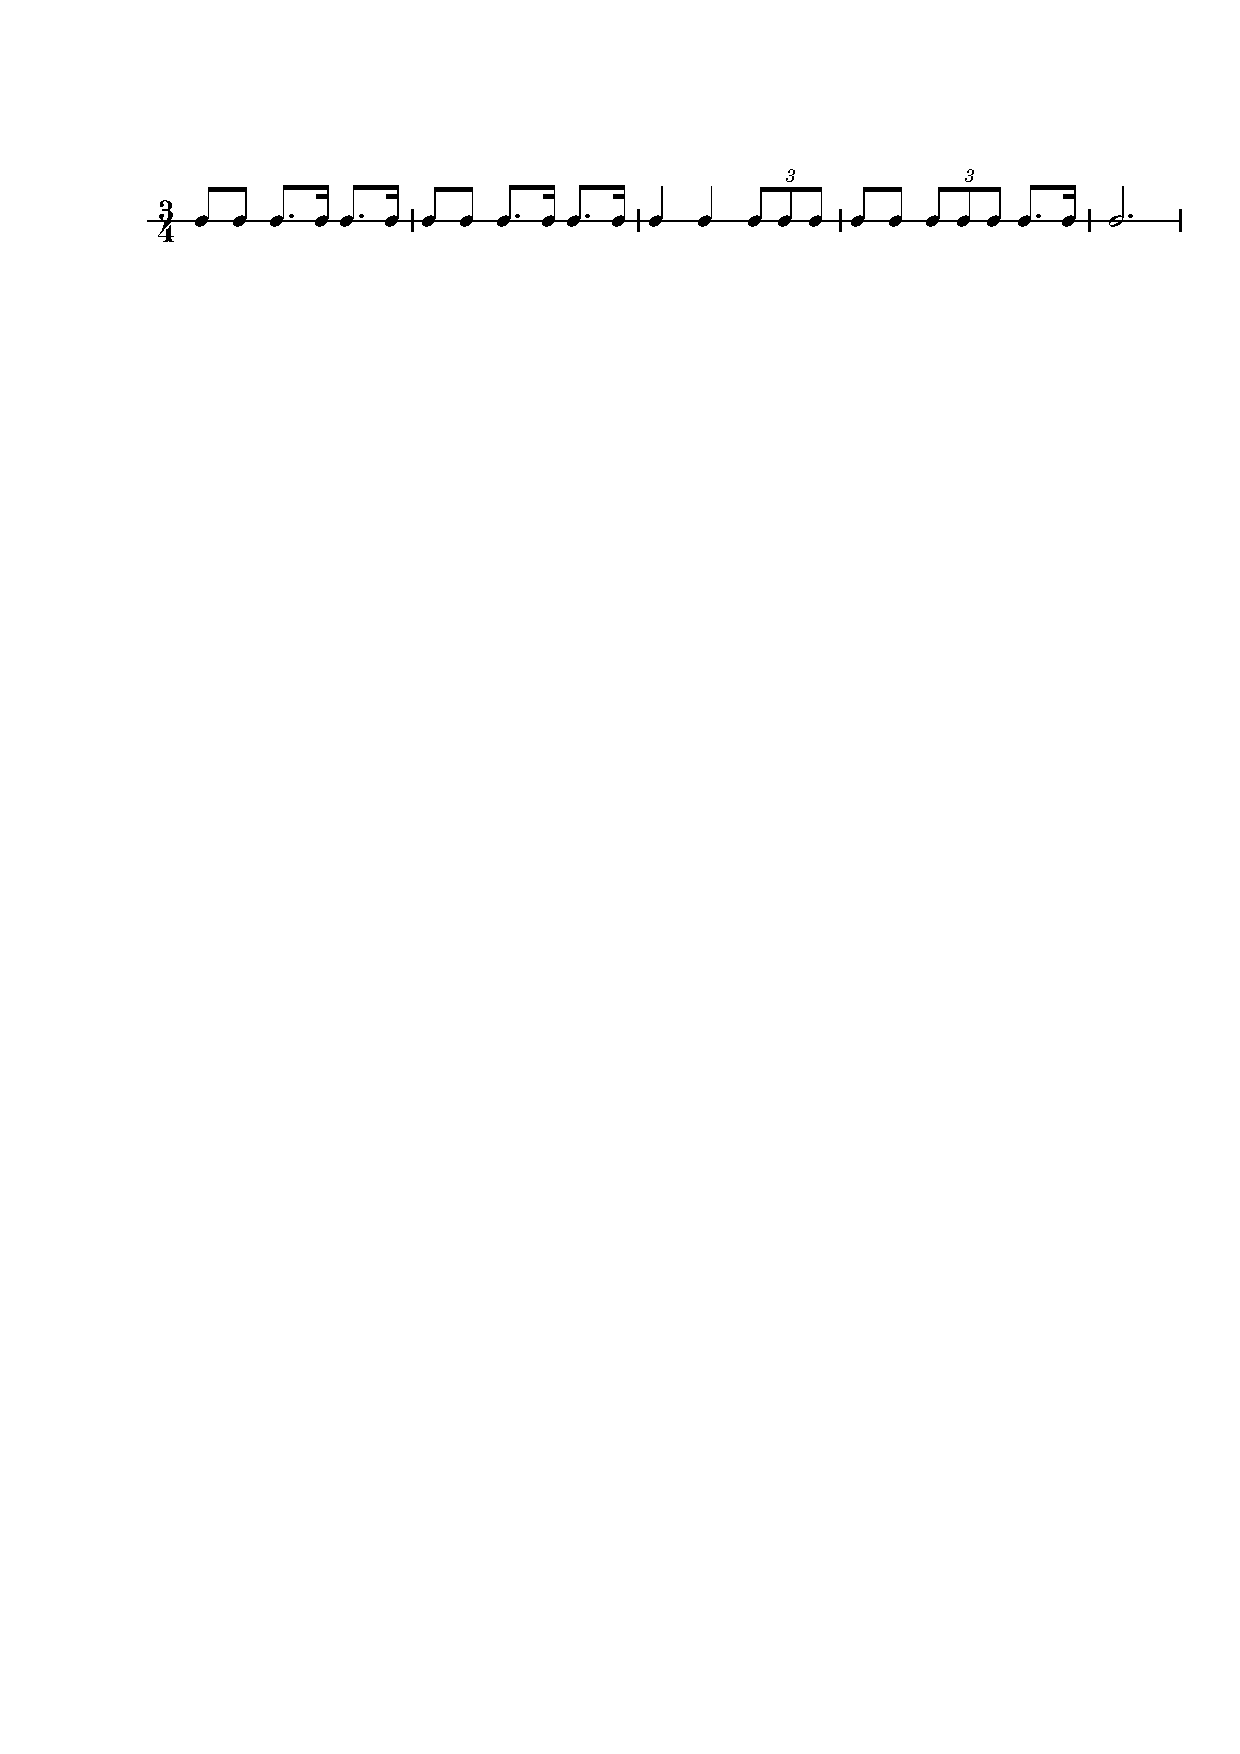
\includegraphics[width=16cm]{3_4_new.pdf}
\caption{A generated passage of 3/4. Note the repetition of measures 1 and 2, a result of variable instantiation during Phase 1 of generation.}\label{example_3_4}
\end{figure*}

\begin{table}
\centering
\begin{tabular}{ll}
1.00 & $M \rightarrow ThreeFour$\\
0.33 & $ThreeFour \rightarrow B^\frac{1}{4} B^\frac{1}{4} B^\frac{1}{4}$\\
0.33 & $ThreeFour \rightarrow \textbf{let} \; x = B^\frac{1}{4} \textbf{in} \; B^\frac{1}{4} x \; x$\\
0.33 & $ThreeFour \rightarrow \textbf{let} \; x = B^\frac{1}{4} \textbf{in} \; x \; x \; B^\frac{1}{4}$\\
\end{tabular}
\caption{Rules used for Phases 2 and 3 to generate Figure \ref{example_3_4}. Rule sets for other phases are omitted here for the sake of brevity.}\label{3_4rules_phases23}
\end{table}

Figure \ref{example_4_4} shows an eight-measure, 4/4 passage generated with the rule sets in Tables \ref{4_4rules_phases123} and \ref{4_4rules}. The rules for the first three phases are trivial: after subdividing the initial $M^8$ symbol into a string of eight $M^1$, each is converted to $FourFour$, and then to $B^1$, a whole note. The nine rules in Table \ref{4_4rules}, which were applied for four iterations, did most of the work. From this small set of rules, we are able to generate a highly varied set of rhythms. For instance, $B \rightarrow D^\frac{3}{4} B^\frac{1}{4}$ has been applied to four distinct durations: a whole note (mm.\ 1-2), a quarter note (mm.\ 1, 3, 6-8), a half note (m.\ 5), and a triplet quarter note (m.\ 8). Although no rule directly subdivides a beat into four or eight notes of the same duration, phenomena like the eight consecutive sixteenth notes in m. 5 are made more probable through the use of let-in rules.

The quarter-note triplet in m.\ 8 of Figure \ref{example_4_4} reveals one drawback of this approach: some subdivision rules are \linebreak more idiomatic than others on larger metrical scales. Because we subdivide with the same rule set each time, each rule has the same likelihood of being applied to a quarter note as it does to a whole note. This presents a difficulty: quintuplet subdivisions, though rare, are sometimes encountered in common practice era music as quick ornamental groupings. Including a rule to generate quintuplets would mean accepting the possibility of a whole note becoming a quarter note quintuplet as well.

This problem could be partially addressed by adding rules to Phase 3 to ensure that a $FourFour$ symbol expands into sensible, larger subdivisions, such as a group of four quarter notes. However, in order to retain the same degree of flexibility, we would have to include many such rules in Phase 3, duplicating the ``acceptable" ways in which a whole note could decompose under the Phase 4 rule set. This is hardly a convincing solution, since we would also be dispensing entirely with the possibility of generating an undivided whole note in the final string. We acknowledge that the present solution--setting the probabilities of rules such as the triplet subdivision to be very low--is the best we can do without modifying the implementation (see Future Work).

In Figure \ref{example_3_4}, we see a 3/4 passage generated by the same grammar. By simply altering a few rules in the early phases of generation, we were able to produce rhythm in a completely different time signature using the same grammar and implementation. Instead of transforming $Measures$ into $FourFour$ symbols, we transform them to \linebreak $ThreeFour$ and then provide a set of possibilities for decomposing a $ThreeFour$ measure into a sequence of \linebreak $Beats$. This justifies our earlier separation of the concept of phrase structure from time signature, and time signature from subdivisions of smaller beats. The rules for Phases 2 and 3 are shown in Table \ref{3_4rules_phases23}; Phases 1 and 4 were unchanged, although the Phase 4 rule set was only applied once.

%%%%%%%%%%%%%%%%% Complex Example %%%%%%%%%%%%%%%%%%

\begin{figure*}[t] % NEEDS REPLACING BUT DEMOS MULTI-COLUMN SPAN
\centering
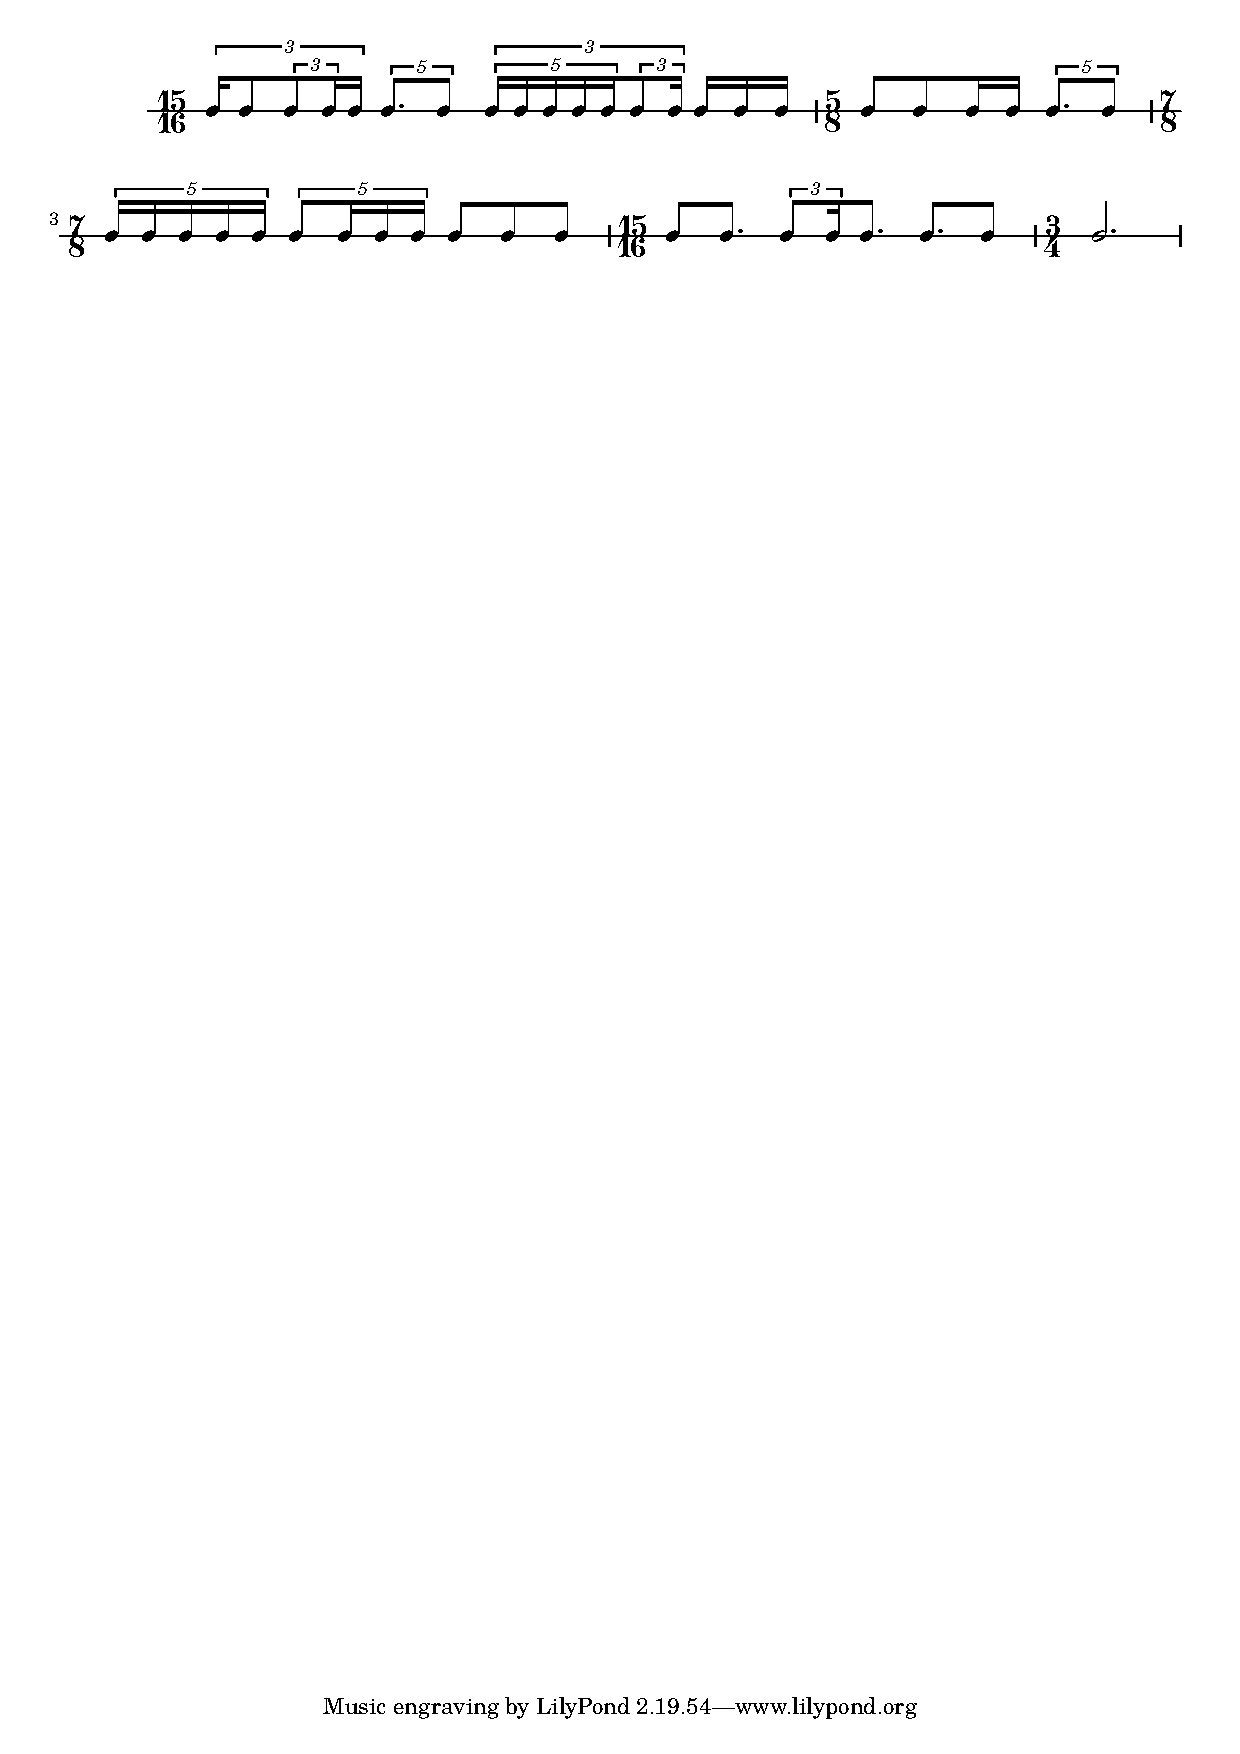
\includegraphics[width=16cm]{complex.pdf}
\caption{A brief passage demonstrating the ability of this framework to easily generate rhythms in multiple time signatures with complex beat subdivisions. A partial rule set is given in Table \ref{complex_rules_phases23}}\label{example_complex}
\end{figure*}

\begin{figure*}[t] % NEEDS REPLACING BUT DEMOS MULTI-COLUMN SPAN
\centering
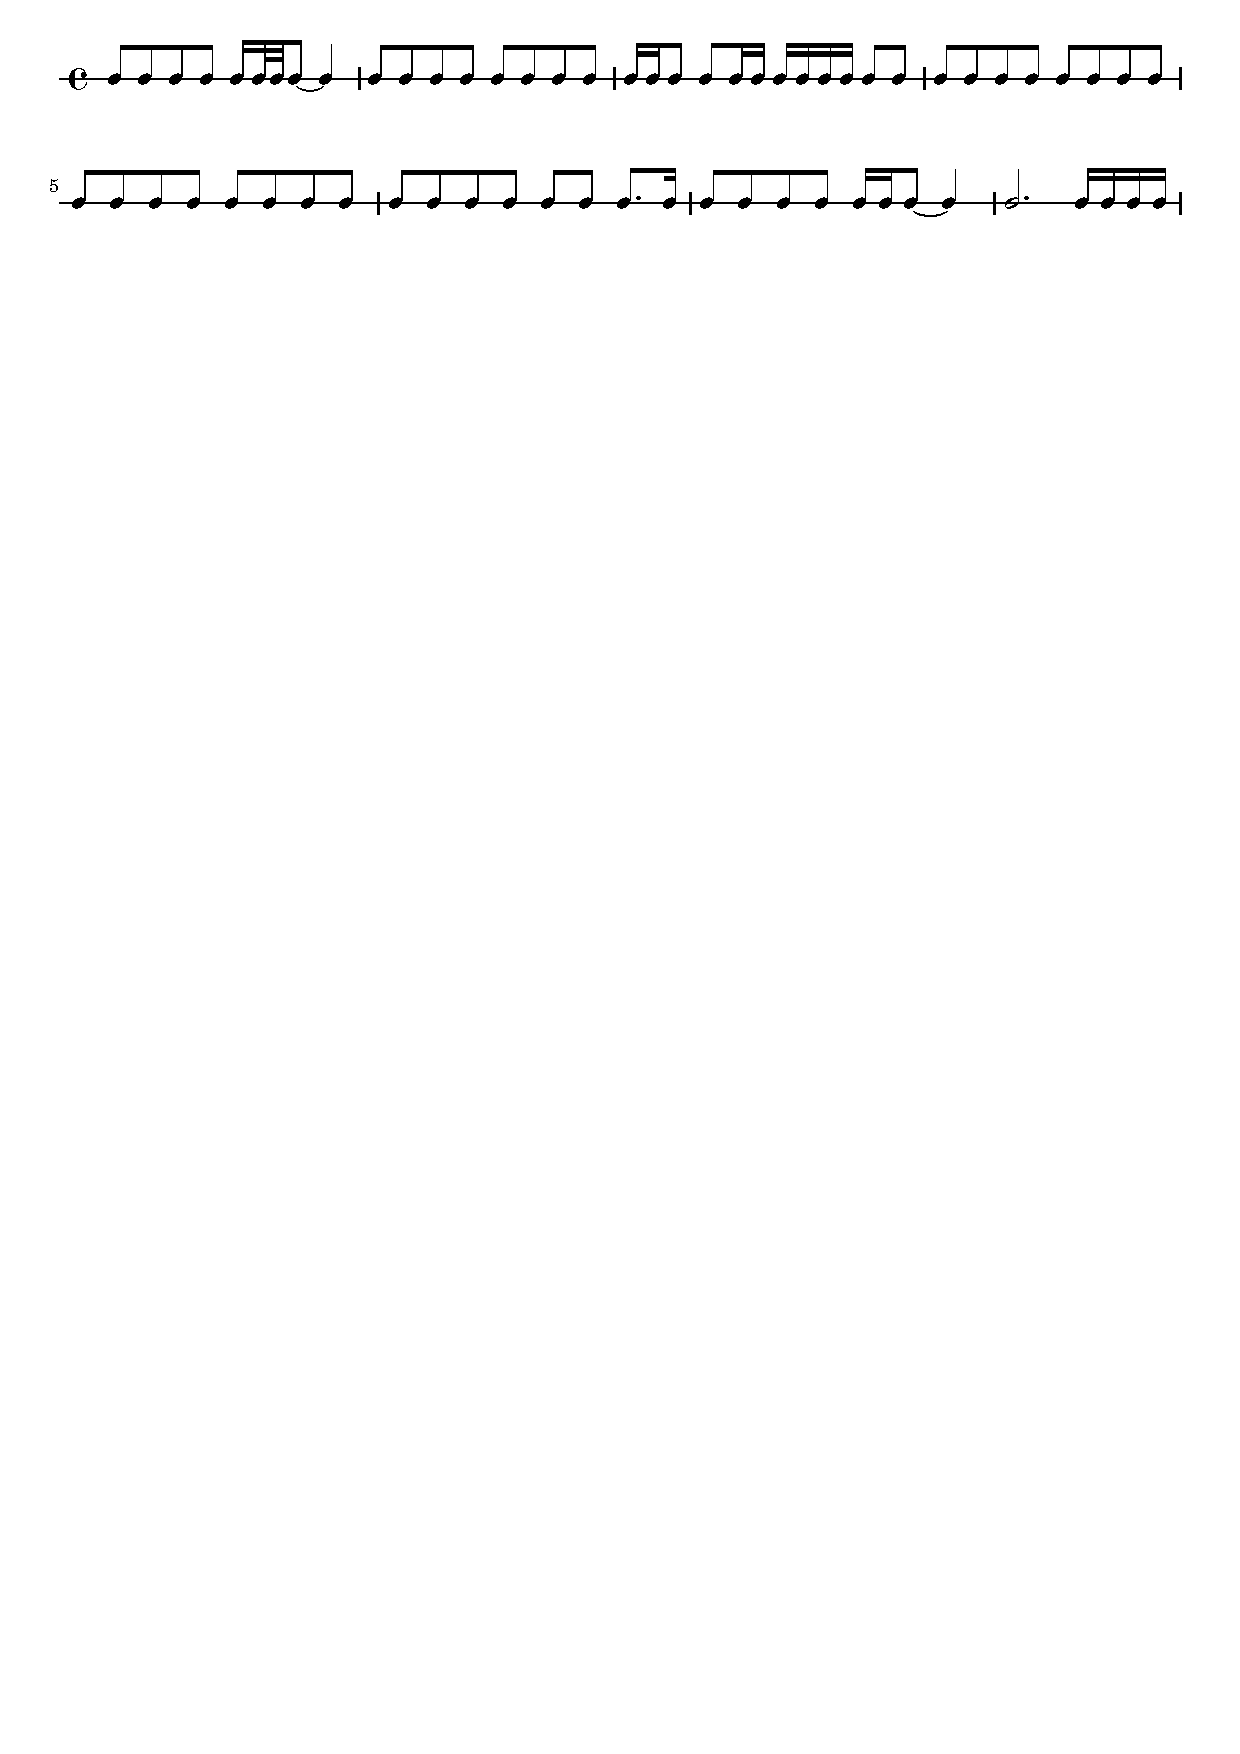
\includegraphics[width=16cm]{bach_output.pdf}
\caption{Examples of rhythms generated from the grammar in Table \ref{simplerules}, the probabilities for which were derived from a small number of Bach cantata excerpts.}\label{learninggen}
\end{figure*}

\begin{table}
\centering
\begin{tabular}{ll}
0.40 & $M \rightarrow FifteenSixteen$\\
0.20 & $M \rightarrow ThreeFour$\\
0.20 & $M \rightarrow FiveEight$\\
0.20 & $M \rightarrow SevenEight$\\
1.00 & $ThreeFour \rightarrow B^\frac{1}{4} B^\frac{1}{4} B^\frac{1}{4}$\\
1.00 & $FiveEight \rightarrow B^\frac{3}{8} B^\frac{1}{4}$\\
1.00 & $FifteenSixteen \rightarrow B^\frac{1}{4} B^\frac{1}{4} B^\frac{1}{4} B^\frac{3}{16}$\\
1.00 & $FifteenSixteen \rightarrow B^\frac{5}{16} B^\frac{5}{16} B^\frac{5}{16}$\\
1.00 & $SevenEight \rightarrow B^\frac{1}{4} B^\frac{1}{4} B^\frac{3}{8}$\\
\end{tabular}
\caption{Rule used for Phases 2 and 3 to generate figure \ref{exmample_complex}. The rule set for Phase 4 has been omitted for the sake of brevity.}\label{complex_rules_phases23}
\end{table}

The previous example diversified the rule set of Phase 3, beat pattern generation. What if we wanted to also diversify Phase 2, time signature assignment? Figure \ref{example_complex} shows an example of this grammar in which an abstract measure is allowed to transform into any one of four time signatures, each of which further transforms into one of potentially multiple beat patterns (Table \ref{complex_rules_phases23}). Considering m.\ 1 of Figure \ref{example_complex}, we note that this grammar, by virtue of its ratio-based representation of duration values, gracefully produces nested tuplets of arbitrary denominator.

In a passage like Figure \ref{example_3_4}, the frequent downbeats and lack of syncopation could quickly become tiresome in a longer passage of 16 or 32 measures. The current model has no way to address this potential for monotony: no matter how a duration is subdivided, the resulting sequence always keeps the initial impulse the same. There are a number of modifications that could be made to the grammar to address this shortcoming (see Future Work).

%%%%%%%%%%%%%%%%%%%%%%%%% Learning %%%%%%%%%%%%%%%%%%%%%%%%%%%%%%%

\section{Learning Production Probabilities}

An algorithm for deriving production probabilities from a training corpus has been described for probabilistic temporal graph grammars \cite{kulitta_learning}, and is part of the Kulitta framework. This learning method is based on the inside-outside algorithm\cite{lari1990}, which, in turn, is a tree generalization of the more commonly used forward-backward algorithm for hidden Markov models.

Kulitta's production probability learning-strategy is \linebreak oracle-based, allowing PTGG for which the oracle can be defined concretely to have production probabilities estimated from real data. This strategy also supports PTGGs with rules that feature let-in expressions and conditional statements. The oracle must be able to identify candidate parent symbols that may have produced mixed sequences of terminals and nonterminals. 

For the PTGGs described in this paper, the learning oracle is simple to define because all of the rules are \emph{duration preserving}. A rule can be tested against a sequence of symbols by normalizing the durations of the input sequence to sum to 1.0 and comparing against symbol parameters in the rule. For example, the sequence $B^{2}B^{2}$, which normalizes to $B \rightarrow B^\frac{1}{2} B^\frac{1}{2}$ can clearly be produced by the rule $B \rightarrow B^\frac{1}{2} B^\frac{1}{2}$, but $B^{1} B^{2}$ cannot. 

As a proof of concept, we tested a reduced rule set using a small collection of rhythmic patterns from Bach cantatas. The production probabilities derived from this experiment are shown in Table \ref{simplerules}, and example rhythms generated from the learned model are shown in Figure \ref{learninggen}.

%  [0.8510911736306143,4.426342216253392e-3,2.9856772830154275e-2,2.3793216219438296e-3,7.110892668979364e-2,1.0e-2,1.0e-2,1.0e-2]
\begin{table}
\centering
\begin{tabular}{ll}
0.851 & $B \rightarrow B^\frac{1}{2} B^\frac{1}{2}$\\
0.004 & $B \rightarrow B^\frac{1}{2} B^\frac{1}{4} B^\frac{1}{4}$\\
0.030 & $B \rightarrow B^\frac{1}{4} B^\frac{1}{2} B^\frac{1}{4}$\\ 
0.002 & $B \rightarrow B^\frac{1}{4} B^\frac{1}{4} B^\frac{1}{2}$\\ 
0.071 & $B \rightarrow D^\frac{3}{4} B^\frac{1}{4}$\\
0.010 & $B \rightarrow B^\frac{1}{4} D^\frac{3}{4}$\\
0.010 & $B \rightarrow B^\frac{1}{4} B^\frac{1}{4} B^\frac{1}{4} B^\frac{1}{4}$\\
0.010 & $B \rightarrow B^\frac{1}{3} B^\frac{1}{3} B^\frac{1}{3}$\\ 
\end{tabular}
\caption{Rule set with probabilities derived from training on examples of rhythms from Bach cantatas.}\label{simplerules}
\end{table}

%\begin{figure}[h]
%\centering
%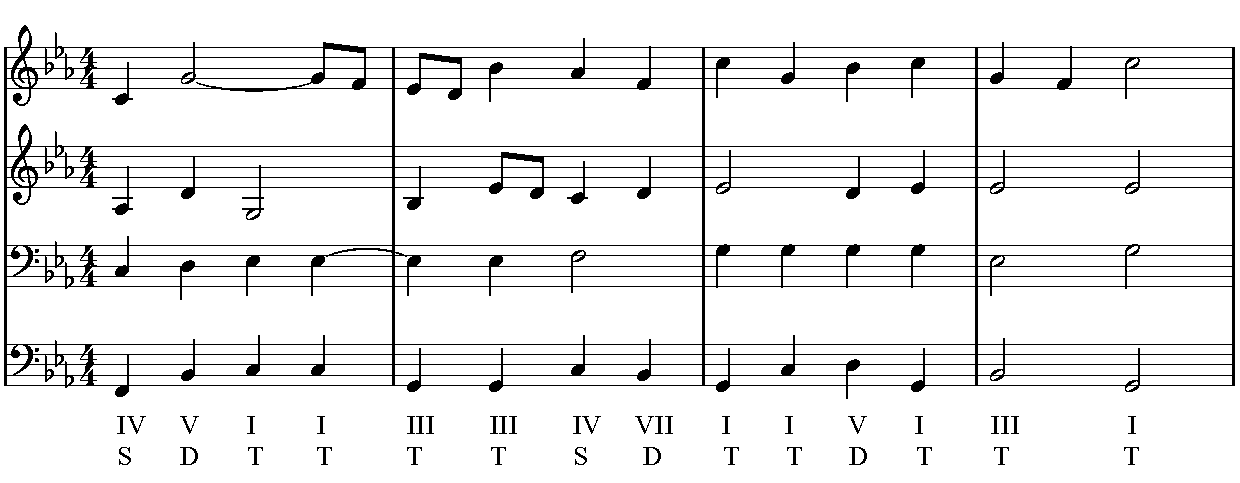
\includegraphics[width=0.9\columnwidth]{Chorale_443576165_minor.pdf}
%\caption{Some caption}
%\end{figure}

%%%%%%%%%%%%%%%%%%%%%%%%% Conclusion %%%%%%%%%%%%%%%%%%%%%%%%%%%%%%%

\section{Conclusion and Future Work} 

We have presented an application of PTGGs to the topic of automated composition along the sole parameter of rhythm, including the implementation of several example grammars. These grammars support multiple time signatures and complex rhythmic patterns while still retaining a strong sense of meter in generated sequences due to the use of a tiered approach to generating sequences that addresses hypermetrical structure. 

However, there are still rhythmic features missing from our models. 
One clear area for expansion would be the introduction of rests and ties, which would give access to syncopation, an important feature in many genres of music, especially jazz. These extensions would motivate the introduction of more alphabet symbols: a Tied symbol, produced from a Beat or Short, could be interpreted as tied over from the previous note during playback. A Rest symbol could be similarly used to eliminate some articulated notes from the interpreted string. 

Other concepts missing from the current alphabet are accents, embellishments and other ornamentations. Accents in particular are important to the perception of meter. Embellishments/ornaments could add short note values before or after more metrically significant beats, and in so doing establish an additional level of metrical hierarchy. A separate way to approach this would be by allowing existing let-in structures in the string to be resolved during or between iterations, rather than at the end of the entire cycle. This would preserve high-level symmetry while allowing for small-scale variations.

% This doesn't seem relevant anymore?
%With certain adaptations, the proposed grammar could generate rhythms in more contemporary styles: for instance, the composition of mixed-meter passages would require a reworking of the first, Measure-based production phase, and might be better generated additively as opposed to recursively. The grammar already supports the complex and nested tuplets which are often found in classical music of the 20th and 21st centuries, and by slackening the imposed constraint on constant total string duration, it might also be able to generate passages in free meter or ?non-geometric? time.

Another direction to explore is context sensitivity. In some cases, it might be helpful to know certain contextual details about a symbol such as: (1) its position within the measure, which typically determines its emphasis (downbeat vs. upbeat), (2) its position within the overall duration of the passage, and (3) whether the passage is increasing or decreasing in rhythmic activity. Otherwise, it is not possible to account for what Schoenberg termed ?the tendency of the smallest notes?\cite{schoenberg}---a phenomenon wherein shorter durations are used more frequently toward the end of a passage or phrase, without adding other constraints to the rule set.

These variations and extensions could also be useful for interfacing our grammar with other automated composition algorithms that produce melodies, harmonies, and \linebreak counterpoint, either by using its output as a blueprint or by including it in a ?composition by committee? approach. In that case, it would be important to embed as much contextual and functional knowledge as possible into the alphabet and the symbol parameters so that other grammars and algorithms can make informed decisions. For example, the knowledge that a downbeat is tied over or that two halves of a phrase have some rhythmic symmetry could be interpreted by a harmonic composition algorithm to produce more contextually aware chord sequences.

%%%%%%%%%%%%%%%%%%%%%%%%%%%%%%%%%%%%%%%%%%%%%%%%%%%%%%%%%%%%%%%%%%%%%%%%%%%%%
%bibliography here
\bibliography{musicbib3}

\end{document}
